\documentclass[aps,prl,reprint,groupedaddress]{revtex4-1}
\usepackage{graphicx}    % Required for inserting images.
\usepackage{amsmath,amssymb,gensymb}  % Advanced math formatting.
\usepackage{float}  % Required to force figure position.
\usepackage{lipsum} % For dummy text.
\usepackage{hyperref}
 

\begin{document}

\title{Calibration of a Three-dimensional Muon Detector Based on Scintillator Binary Optical Encoding\\[0.5ex] \small Team Dawson Technicolor}

\author{Milo Belarbi}
\author{David Birnbaum}
\author{Tykhon Byshkin}
\author{Matvey Chirchikov}
\author{Danah Dézémé}
\author{Arij Mohamedi} 
\author{Evan Parasol}
\author{Leandro Perez Moran}
\author{Ari Polterovich}
\author{Tian Yi Xia}
\author{Chun On Yu}
\author{Aljoscha Ziegler}
\author{Manuel Toharia}
\altaffiliation{Teacher}
\author{Joel Trudeau}
\altaffiliation{Teacher}

\affiliation{Dawson College, Montreal, Quebec, Canada}
\date{April 10, 2025}

\maketitle



%\begin{multicols}{2}

\section{Introduction}
[Overview of the theory] \\ 

While we have developed the detector’s software and hardware components, precise calibration would require exposure to a controlled muon beam. Access to CERN’s world class facilities would allow us to validate our detector’s performance and refine its accuracy. It would also provide invaluable insights into innovative techniques that would contribute to the broader field of particle detection technology. We hope to collaborate with peers and experts at CERN to deepen our comprehension of physics concepts through real-world applications. We are also committed to inspiring other young Canadian scientists by sharing our experiences and findings through outreach activities. An opportunity to conduct our experiment at CERN would be a pivotal step in this journey. \\ 

[Possible applications]


\section{Design}

The general working principle of our detector is simple:
polyvinyl toluene (PVT) scintillator rods are arranged in
the detector, and when a muon passes through a rod, photons emitted are then detected by a Silicon Photomultiplier
(SiPM). The collected data is then transferred to a computer where the data is processed and rendered to display the possible paths of the muon. Our design strays from conventional detectors when it comes to the arrangement of the scintillator rods. While typical detectors use a grid design, we opted for a design inspired by binary encoding (see figure \ref{fig0}). 


\begin{figure}[h]
    \centering
    \includegraphics[scale=0.46]{figures/sandwich good.png}
\caption{Comparison of three scintillator placement methods: $n$ being the number of scintillators on the side of
one of the extreme layers. 
\textbf{Left:} One layer grid design. Number of sensors scale as $2n^2$.
\textbf{Middle:} Two layer grid design, scales as $4n$.
\textbf{Right:} Binary
encoding arrangement, number of required sensors scales as
$8 log_2(n)$. In each layer, identically coloured
scintillators are optically linked to the same SiPM by WLS
fiber.}
\label{fig0}
\end{figure}



This has two main benefits. First, it reduces the number of sensors needed, as only two sensors are necessary per layer. As such, the number of sensors needed for the detector increases logarithmically. Our design also allows for easy encoding of the detector’s state. With each layer only having two sensors, its state can be represented with a single bit, and because each layer is more specific than the previous, it narrows down the possible paths of the particle through the detector. Each set of signals therefore encodes for a specific pattern. This is analogous to the system used in the Apollo Guidance Computer’s rope core memory, with each bit representing an inhibit wire pair\cite{agc}.


\begin{figure}[h]
    \centering
    \includegraphics[scale=0.65]{figures/bare rods.png}
    \caption{Isometric view of physical detector. WLS fiber is encased within dark tubing toward the SiPM boards. Four threaded rods elevate the top platform: nuts allow for relative parallelism adjustment. Top and bottom scintillator packs permit the encoding of XY positioning; both combined, 3D trajectory tracking. A total of $12\,\text{layers} \times 2\,\text{SiPMs/layer} = 24\,\text{SiPMs}$.}
    \label{fig1}
\end{figure}

%\clearpage

\vspace{10mm}
In greater detail, each rod is optically isolated from its neighbors with aluminium foil and connected to a remote SiPM through wavelength shifting fiber (WLS fiber)\cite{wls} . We opted for WLS fiber, as is common among scintillation detectors, because it is more efficient at capturing the photons emitted by the scintillators than clear fibers. The output of the SiPMs being too weak, we use op-amp transimpedance amplifiers to amplify the signal. After being amplified, the signals are digitized before entering an FPGA circuit for fast acquisition \footnote{All circuits and PCBs are custom-made. Access the documentation \href{https://github.com/ThatAquarel/hep/tree/main/scintillator_field/hardware/docs}{\underline{here}}}. An Arduino then filters the signal before it is sent to a computer for processing.


\begin{figure}[h]
    \centering
    \includegraphics[scale=0.28]{figures/fig2.JPG}
\caption{Student-designed SiPM printed-circuit boards. Each PCB has four channels; a total of six PCBs are used in our detector. SiPMs and other components are manually populated onto the PCB.}
\label{fig2}
\end{figure}

%BIG BOX
\begin{figure} [h]
    \centering
    \includegraphics[scale=0.097]{figures/big detector.jpg}
    \caption{Binary optical encoding scintillation detector in its final form. \textbf{Left:} Light-tight faraday cage containing the detector made of HVAC conduit\textemdash decreasing light contamination and electrical noise. \textbf{Right:} Acquisition circuit linked with data cables.}
    \label{fig4}
\end{figure}

\vspace{15mm}
The trajectory volume\textemdash the possible volume of muon trajectory\textemdash is calculated in O(n) using Python code\footnote{All code can be found in our \href{https://github.com/ThatAquarel/hep}{\underline{GitHub repository}}.} by splitting the detector into two side-projections. The code calculates the trajectory volume projection for each side view by iterating over two levels at a time and conserving the tightest projection, first combining the center levels and finally the uppermost and lowermost levels. The volume trajectory projections are combined into the volume trajectory. Future updates will include : adapting to situations where the muon passed between two rods of the same level and taking advantage of situations where muons had to pass in between same level rods. 

 

\begin{figure}[h]
    \centering
    \includegraphics[scale=0.85]{figures/fig3_cropped.png}
    \caption{Representation of a possible muon trajectory and the calculated trajectory volume projection. Black line a possible muon path. Black dotted line is the side muon volume projection: boundaries for all possible muon paths.
}
    \label{fig3}
\end{figure}


The display is written in Python, using GLFW to create the display window, PyOpenGL to turn the coordinates from the muon volume trajectory into coordinates relevant to the computer, as well as to create the shaders, vertex arrays, and vertex buffers which are needed to render the scintillator structure and trajectory volume to the computer, and ImGui to create the text box that gives information to users.
\begin{figure}[h]
    \centering
    \includegraphics[scale=0.5]{figures/fig4.png}
    \caption{Two experimental instances of isometric views of binary positional decoding by our software from real data. \textbf{Left:} Signals sent to the computer are interpreted visually. \textbf{\textit{Yellow:}} Triggered scintillators. \textbf{\textit{White:}} Untriggered scintillators. \textbf{\textit{Red:}} Volume of possible muon trajectory resulting from binary elimination of trajectories. \textbf{Right:} More efficient render without signal interpretation. \textbf{\textit{Purple:}} Volume of possible muon trajectories.}
    \label{fig4}
\end{figure}


\vspace{40mm}
\section{Results}
After initial testing, we recorded several detections. The results were not affected by the intensity of light in the room, suggesting that the detector was successfully optically sealed.

The muon flux detected is around 2.5 hits/minute, lower than in theory. We believe that this is due to our conservative data filtering, and small field of view: we wanted to reduce the chances of introducing noise as much as possible. As such, the calibration of our detector is crucial to capture accurate trajectories.


%oscilloscope 1
\begin{figure} [h]
    \centering
    \includegraphics[width=0.58\linewidth]{figures/scope_yellow_green.png}
    \caption{Initial amplification testing with OnSemi C-Series SiPM (41\% photon detection efficiency (PDE), 420\,nm peak wavelength). \textbf{Yellow:} voltage across $49.9\,\Omega \pm 1\%$ shunt resistor on reverse-biased diode anode. \textbf{Green:} non-inverting op-amp configuration (LT1807) output. Light output measured from BC408 PVT scintillator.
}
    \label{fig3}
\end{figure}



%oscilloscope 2
\begin{figure} [h]
    \centering
    \includegraphics[width=0.58\linewidth]{figures/scope_yellow_purple.png}
    \caption{Initial transimpedance amplifier testing. Gain of $2.26 \times 10^5 \pm 1\%$. \textbf{Yellow:} inverting op-amp output. \textbf{Pink:} low-pass filter, 940\,kHz bandwidth.}
    \label{fig4}
\end{figure}

%Angle model
\begin{figure} [h]
    \centering
    \includegraphics[scale=0.45]{figures/angle fig2.png}
    \caption{Cosmic ray capturing field of view: $46\pm2\degree$ minimum (on X and Y axes side projection), $62\pm2\degree$ maximum (on diagonal). Top and bottom scintillator stacks are $140\times140\times90 \pm2.5$ mm\textemdash separated by an air-gap of $162 \pm1$ mm. The minimum trajectory volume cross-section is $15\times15\text{ mm}: 225\text{ mm}^2$.}
    \label{angles}
\end{figure}



%\clearpage

\section{Experimental Proposal}
Our muon tracker is currently producing experimental results, but we have no way of confirming their validity. As such, we propose using CERN’s high-energy Proton Synchrotron as a source of a controlled muon beam and use this experiment to compare our detector tracking results with the known trajectory of the Proton Synchrotron muon beam.

The evaluation of XY translational accuracy will be assessed by aiming the detector’s Z axis toward the beamline and iterating through different XY positions; the evaluation of XYZ rotational accuracy will be done by iterating through diverse altitude and azimuth angles. As the position is encoded to an $8 \times 8$ grid, a minimum of 64 different translations and 64 rotations will confirm the correct triggering of all SiPMs and the faithfulness of the trajectory volume computation with the actual trajectories.
\begin{figure} [h]
    \centering
    \includegraphics[scale=0.2]{figures/proposed test.png}
    \caption{Experimental proposal axes reference frame. \textbf{Left:} Example XY translational testing beamlines. \textbf{Right:} Example XYZ rotational testing beamlines.}
    \label{proposed tests}
\end{figure}

\begin{figure} [h]
    \centering
    \includegraphics[width=0.58\linewidth]{figures/digitizer all.png}
    \caption{Digitizer circuit signals from acquisition hardware. \textbf{Yellow:} analog output from trans-impedance amplifier connected to comparator inverting input. \textbf{Red:} latching FPGA register for acquisition. \textbf{Blue:} comparator output. \textbf{Green:} level-shifted comparator output. Adjustable comparator threshold voltage: 1.133V $\pm$ 0.1\%.}
    \label{digitizer}
\end{figure}

\section{Outlook}
We have fully developed the detector’s software and hardware components on our own. Therefore, precise calibration would require exposure to a controlled muon beam. Further, a controlled muon beam would permit us to test out features we are currently developing such as measuring the detection time and using a time-over-threshold system to find the energy of muons passing through the detector. Access to CERN’s facilities would allow us to validate our detector’s performance and refine its accuracy.

The confirmation of the viability at CERN of our safety-oriented detector design allows for open-sourcing, along with physics classroom outreach—projects with which we align. We believe that getting this detector ready for research will inspire more students to design their own particle physics experiments.


%TC:ignore
\section{Community outreach}
Women, though largely unrecognized, have played a great role in the development of modern science. Marie Curie, Ada Lovelace, Katherine Johnson, and many others have been role models for generations of scientists. Our team at Dawson TECHNICOLOR firmly believes that part of promoting science education is promoting the inclusion of women and other marginalized groups. As such, we are currently working with Dawson STEMM FEM, a local club, to create talks and participate in events that will hopefully encourage many young women to join the beautiful field of physics and of science as a whole.

Furthermore, The Scintillating Chamber is set to be presented in May at Dawson’s ScienceFest. This event consists of a fair where a myriad of scientific projects are introduced to the student body. This opportunity will allow us to make particle physics more accessible and easier to grasp while sharing our unwavering passion.

%\end{multicols}

% Section: Acknowledgements
%\clearpage
\section{Acknowledgments}
\begin{center}
    \textbf{Acknowledgements}
\end{center}

We would like to sincerely thank Dr. Manuel Toharia for his dedication to the High Energy Particle Physics group at Dawson, for his captivating lectures and for his guidance throughout our project. We are incredibly grateful to McGill University Professor Dr. François Corriveau for his guidance as well as McGill Professor Dr. David Hanna for his invaluable advice and for graciously letting us use his scintillator block. We express our sincere appreciation to Université de Montréal technician Dr. Nikolai Starinsky for his scintillator cutting advice. This project would not have been possible without the Dawson Foundation’s Student Academic Growth and Enrichment Fund, who’s grant provided money with which we bought power tools, safety equipment, and electronics. Finally, we would like to express our gratitude to Dawson College for offering us a wonderful learning environment that allowed us to flourish and engage in science activities that we are passionate about. 


\clearpage
\section{Appendices}
\begin{figure} [h]
    \centering
    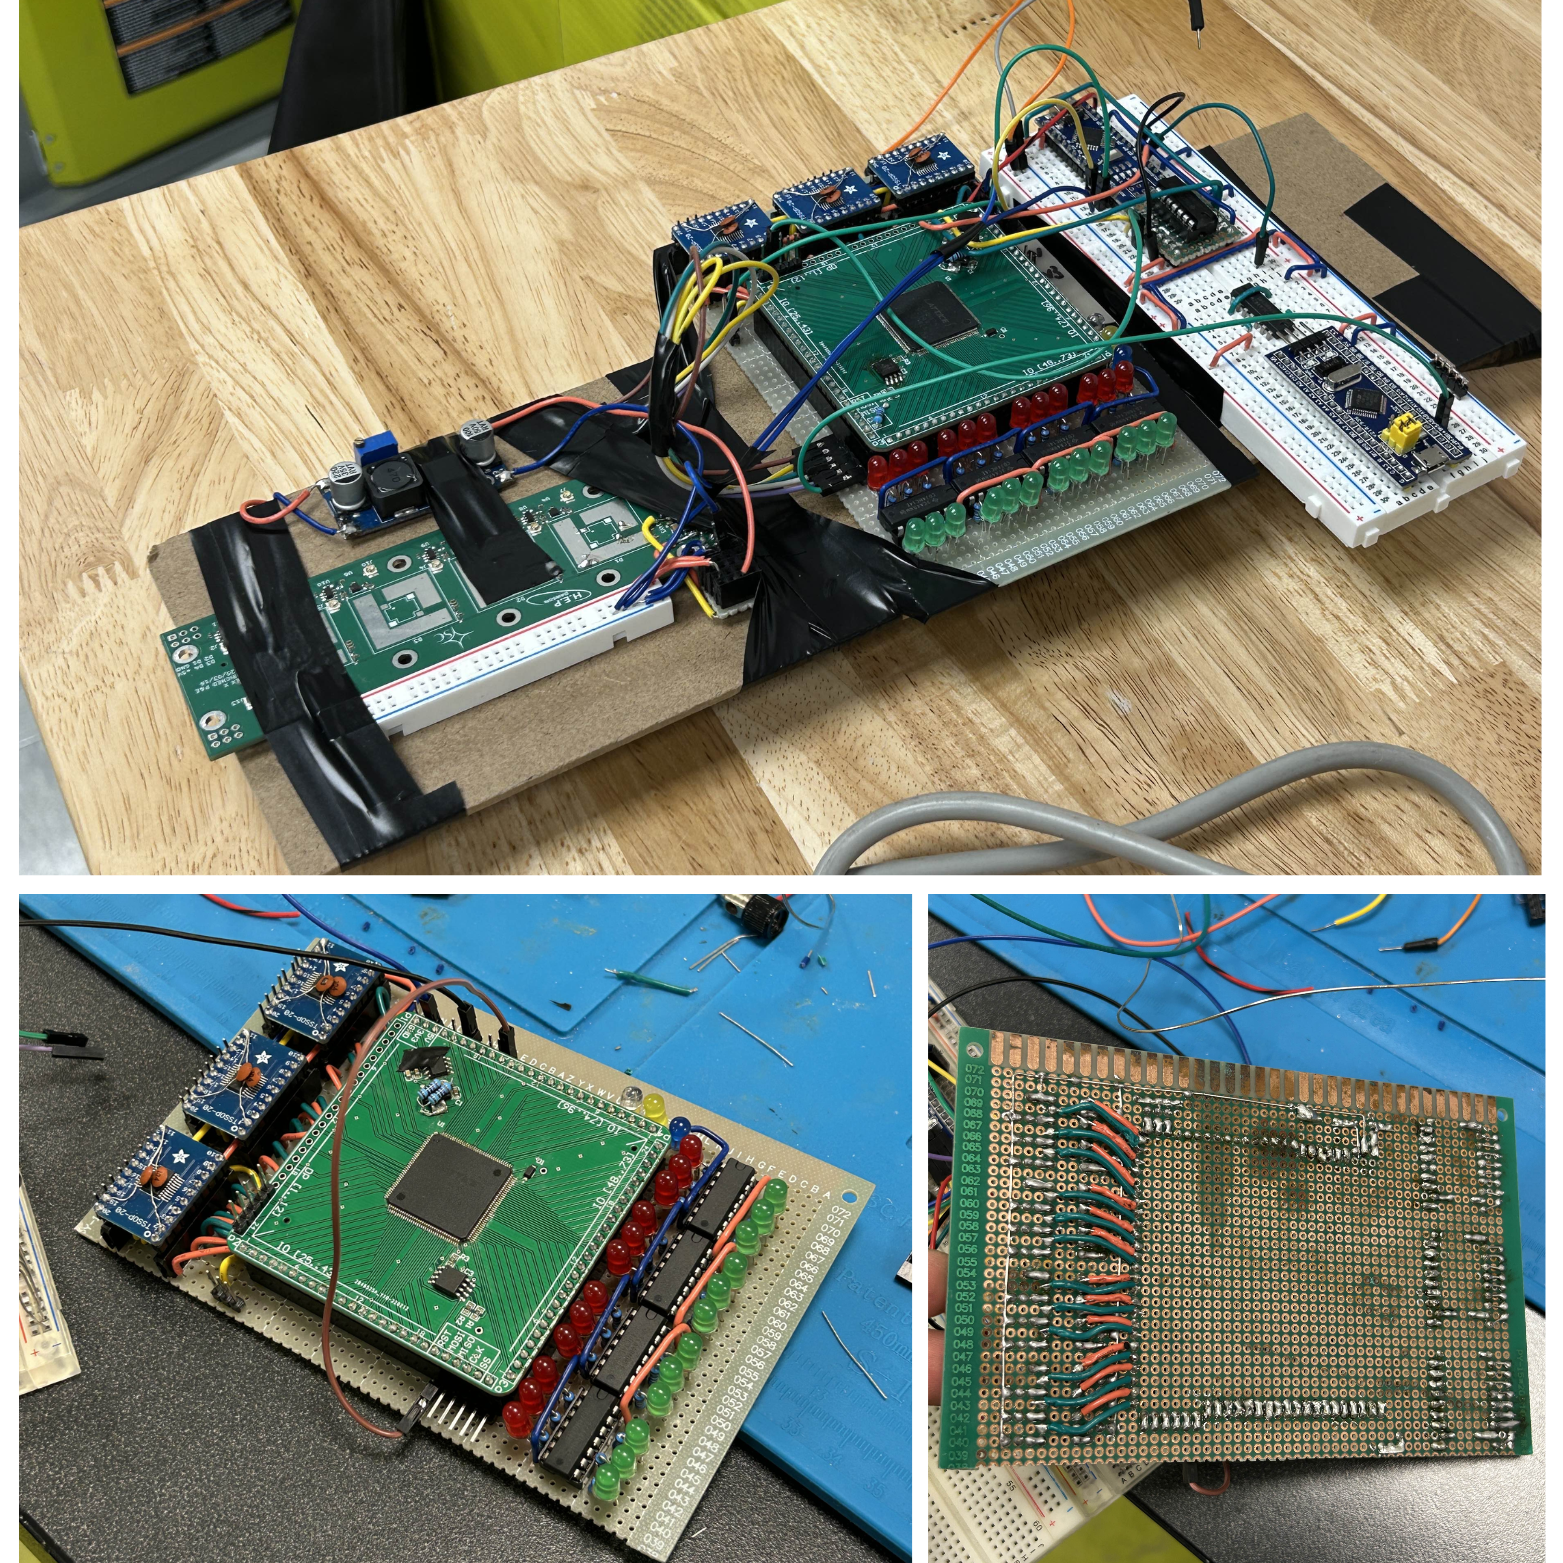
\includegraphics[scale=0.5]{figures/fig5.png}
    \caption{\textbf{Top:} Signal acquisition circuit. \textbf{\textit{Left:}} Low-noise 5\,V power supply for all SiPM PCB boards (TPS7A470, $4\,\mu\text{V}_\text{RMS}$). \textbf{\textit{Middle:}} 24-channel digital signal reader with FPGA (ICE40HX1K), 5\,V to 3.3\,V level shifters, and indicator LEDs associated with each SiPM sensor. \textbf{\textit{Right:}} Breadboard: Arduino Nano for serial data communication over USB to the computer, and STM32F103C for clock signal generation. \textbf{Bottom left:} Work in progress FPGA detector module. \textbf{Bottom right:} Manual soldering of individual wires for the 24 LED indicators.}
    \label{fig5}
\end{figure}


\begin{figure}[h] 
    \centering 
    \includegraphics[scale=0.6]{figures/fig6.png}
    \caption{Scintillator rods cut with a bandsaw from a larger
scintillator block. Two $500\times250\times30$ mm BC408 PVT scintillators were graciously offered to us by McGill Professor Dr. David Hanna\textemdash which we then proceeded to cut and polish manually.}
    \label{fig6}
\end{figure}





\begin{thebibliography}{99}
% \cite{Spectrum of CRM}
\bibitem{Spectrum of CRM}
Gardner, M., et al., "The Momentum Spectrum of Cosmic Ray Muons near Sea Level in the Momentum Range 0.4--10 GeV/c." IOPScience. Accessed March 2022,
\url{https://iopscience.iop.org/article/10.1088/0370-1328/80/3/314/pdf}.

% \cite{hyperphysics}
\bibitem{hyperphysics}
Hyperphysics, "Atmospheric Muons." Georgia State University. Accessed March 2022,
\url{http://hyperphysics.phy-astr.gsu.edu/hbase/Particles/muonatm.html}.

% \cite{atmospheric muon}
\bibitem{atmospheric muon}
CERN, "Cosmic Rays: Particles from Outer Space." Accessed March 2022,
\url{https://home.cern/science/physics/cosmic-rays-particles-outer-space}.

\bibitem{pdg}
K.~Nakamura \textit{et al.} [Particle Data Group], J. Phys. G \textbf{37}, 075021 (2010),
doi:10.1088/0954-3899/37/7A/075021,
\url{https://pdg.lbl.gov/2011/reviews/rpp2011-rev-cosmic-rays.pdf}.



\bibitem{agc}
Kuttner, P. The rope memory: a permanent storage device. {\em Proceedings Of The November 12-14, 1963, Fall Joint Computer Conference}. pp. 45-57 (1963), \url{https://doi.org/10.1145/1463822.1463829}


\bibitem{wls}Worstell, W., Doulas, S., Johnson, O. \& Lin, C. Scintillator crystal readout with wavelength-shifting optical fibers. {\em Proceedings Of 1994 IEEE Nuclear Science Symposium - NSS'94}. \textbf{4} pp. 1869-1873 vol.4 (1994)
\url{https://dl.acm.org/doi/pdf/10.1145/1463822.1463829}


\end{thebibliography}
%TC:endignore

\end{document}